\chapter{Calgary 实验结果}

最简单的傅里叶变换成像重建方法,采用2D IFFT,全采样数据


\begin{figure}[H]
    \centering
    \includegraphics[width=0.6\linewidth]{fig/coil1.png}
    \caption{第1个线圈}
    \label{fig:coil1}
\end{figure}


\begin{figure}[H]
    \centering
    \includegraphics[width=0.6\linewidth]{fig/coil2.png}
    \caption{第2个线圈}
    \label{fig:coil2}
\end{figure}


\begin{figure}[H]
    \centering
    \includegraphics[width=0.6\linewidth]{fig/coil3.png}
    \caption{第3个线圈}
    \label{fig:coil3}
\end{figure}


\begin{figure}[H]
    \centering
    \includegraphics[width=0.6\linewidth]{fig/coil4.png}
    \caption{第4个线圈}
    \label{fig:coil4}
\end{figure}


\begin{figure}[H]
    \centering
    \includegraphics[width=0.6\linewidth]{fig/coil5.png}
    \caption{第5个线圈}
    \label{fig:coil5}
\end{figure}


\begin{figure}[H]
    \centering
    \includegraphics[width=0.6\linewidth]{fig/coil6.png}
    \caption{第6个线圈}
    \label{fig:coil6}
\end{figure}



\begin{figure}[H]
    \centering
    \includegraphics[width=0.6\linewidth]{fig/coil7.png}
    \caption{第7个线圈}
    \label{fig:coil7}
\end{figure}


\begin{figure}[H]
    \centering
    \includegraphics[width=0.6\linewidth]{fig/coil8.png}
    \caption{第8个线圈}
    \label{fig:coil8}
\end{figure}


\begin{figure}[H]
    \centering
    \includegraphics[width=0.6\linewidth]{fig/coil9.png}
    \caption{第9个线圈}
    \label{fig:coil9}
\end{figure}


\begin{figure}[H]
    \centering
    \includegraphics[width=0.6\linewidth]{fig/coil10.png}
    \caption{第10个线圈}
    \label{fig:coil10}
\end{figure}


\begin{figure}[H]
    \centering
    \includegraphics[width=0.6\linewidth]{fig/coil11.png}
    \caption{第11个线圈}
    \label{fig:coil11}
\end{figure}


\begin{figure}[H]
    \centering
    \includegraphics[width=0.6\linewidth]{fig/coil12.png}
    \caption{第12个线圈}
    \label{fig:coil12}
\end{figure}



\begin{figure}[H]
    \centering
    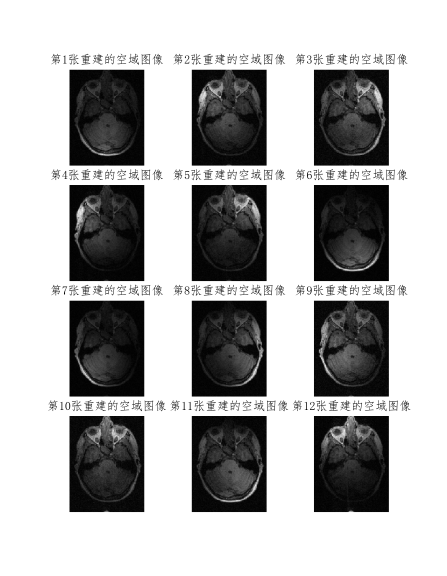
\includegraphics[width=1\linewidth]{fig/12image.png}
    \caption{12个线圈傅里叶变换重建方法结果}
    \label{fig:coil12recon}
\end{figure}


svg图像对比
\begin{figure}[H]
    \centering
    % 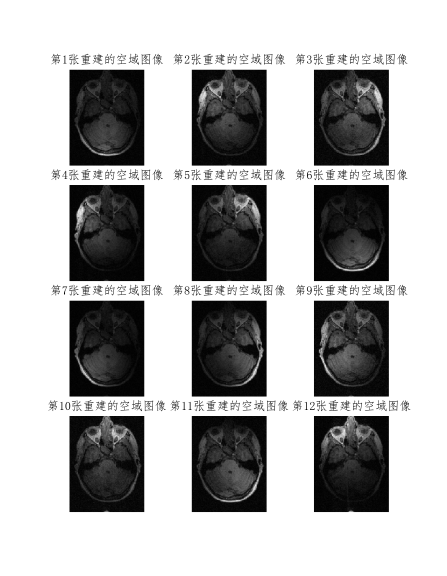
\includegraphics[width=1\linewidth]{fig/12image.png}
    \includesvg[width=1\linewidth]{fig/12image.svg}
    \caption{svg 12个线圈傅里叶变换重建方法结果}
    \label{fig:coil12recon svg}
\end{figure}


\begin{figure}[H]
    \centering
    \includegraphics[width=1\linewidth]{fig/12coil_recon_image.png}
    \caption{12个线圈傅里叶变换重建方法结果}
    \label{fig:coil12recon1}
\end{figure}



\begin{figure}[H]
    \centering
    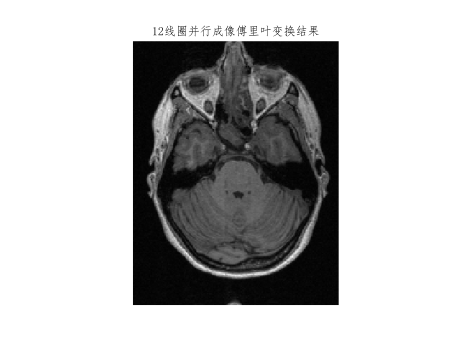
\includegraphics[width=1\linewidth]{fig/12coil_pi_recon.png}
    \caption{12线圈并行成像傅里叶变换重建方法结果}
    \label{fig:coil12_pi_recon}
\end{figure}

svg图像对比
\begin{figure}[H]
    \centering
    % 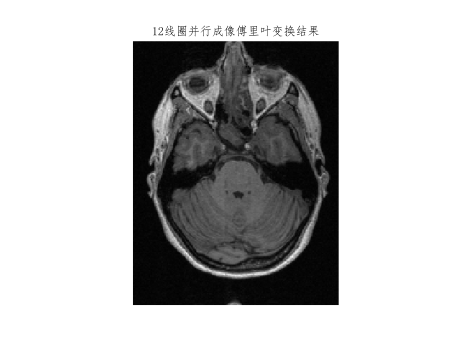
\includegraphics[width=1\linewidth]{fig/12coil_pi_recon.png}
    \includesvg[width=1\linewidth]{fig/12coil_pi_recon.svg}
    \caption{12线圈并行成像傅里叶变换重建方法结果}
    \label{fig:coil12_pi_reconsvg}
\end{figure}


